\documentclass[12pt]{article}

\usepackage[document]{ragged2e}
\usepackage{amsmath}
\usepackage{amssymb}
\usepackage{graphicx}
\usepackage{hyperref}
\usepackage{listings}
\usepackage{color}
\usepackage{textcomp}
\definecolor{listinggray}{gray}{0.9}
\definecolor{lbcolor}{rgb}{0.9,0.9,0.9}
\lstset{
	backgroundcolor=\color{lbcolor},
	tabsize=4,
	rulecolor=,
	language=matlab,
        basicstyle=\scriptsize,
        upquote=true,
        aboveskip={1.5\baselineskip},
        columns=fixed,
        showstringspaces=false,
        extendedchars=true,
        breaklines=true,
        prebreak = \raisebox{0ex}[0ex][0ex]{\ensuremath{\hookleftarrow}},
        frame=single,
        showtabs=false,
        showspaces=false,
        showstringspaces=false,
        identifierstyle=\ttfamily,
        keywordstyle=\color[rgb]{0,0,1},
        commentstyle=\color[rgb]{0.133,0.545,0.133},
        stringstyle=\color[rgb]{0.627,0.126,0.941},
}

\lstdefinelanguage{scala}{
  morekeywords={abstract,case,catch,class,def,%
    do,else,extends,false,final,finally,%
    for,if,implicit,import,match,mixin,%
    new,null,object,override,package,%
    private,protected,requires,return,sealed,%
    super,this,throw,trait,true,try,%
    type,val,var,while,with,yield},
  otherkeywords={=>,<-,<\%,<:,>:,\#,@},
  sensitive=true,
  morecomment=[l]{//},
  morecomment=[n]{/*}{*/},
  morestring=[b]",
  morestring=[b]',
  morestring=[b]"""
}


\author{Jiri Hamberg 013881339}
\title{Distributed Systems Project, Assignment 3}


\newcommand{\norm}[1]{\left\lVert#1\right\rVert}

\begin{document}

\maketitle


\section{ Assignment }

In this assignment we were asked complete three tasks (from the assignment sheet):

\begin{enumerate}

	\item Write	 a	 web-based	 calculator	 which	 uses	 a	 simple	 input	 form	 and	
performs	all	the	calculation	on	the	server	side.
	\item Migrate	some	of	the	functionality	of	the	calculator	to	the	client	side	using	
Javascript.
	\item Implement	caching	of	results	on	the	client	side. 
\end{enumerate}

The application is hosted on a Raspberry pi computer running an Apache Tomcat web server. The application can be reached at 88.115.18.57/calculator. The project also has \href{https://github.com/JiriHamberg/DistSysProj_calculator}{a Github page}. To build the project using SBT (Scala Build Tool), simply run \textit{sbt package} on the root of the project folder. This will create a .war package that is ready to be deployed.

\section{ Implementation }

\subsection*{Task 1}

I chose to use Scalatra web framework for implementing the server since I have some prior experience working with Scala and the framework. The server side functionality of this step is very simple. The following section of code, from CalculatorServlet.scala, registers a handler for HTTP GET requests coming to URL "/calculator". 

\begin{lstlisting}[language=scala]
  get("/calculator") {
  	val (arg1, arg2, op) = (
  		Try(params("arg1").toDouble).toOption,
  		Try(params("arg2").toDouble).toOption,
  		Try(params("op")).toOption
	)

	if(Seq(arg1, arg2, op).forall(p => p.isDefined)) {
		val result: Option[Double] = Calculator.calculate(op.get, arg1.get, arg2.get)
		if (result.isDefined) {
			contentType = "text/plain"
			result.get.toString
		} else {
			BadRequest(reason="Arithmetic error or invalid operator")
		}
	} else {
		BadRequest(reason="Bad parameters")
	} 	
  }    
\end{lstlisting}

If the request has required parameters, then a Calculator service will do the calculation and the result is then sent as the body of the HTTP response. 

The client side of this task is implemented in the Calculator.js file. When the user gives a calculation to the input and hits the "Calculate"-button, the input string will be parsed to a list of operands and operators. The list is then evaluated by repeatedly taking the first three elements of the list and sending them to the server to be calculated and putting the result to the beginning of the list.


\subsection*{Task 2}

The variant of the plotting can be selected with the radio buttons "Server", "Client" and "Cooperative" on the web application. The sine plotting is initiated when the user inputs "sin(x)" and hits the "Calculate"-button.

The server side variant is implemented using gnuplot. The cooperative variant uses a Taylor series expansion of the sine function for approximation. A Taylor polynomial of degree 7 is calculated, sending each individual operation to the server. The operations are chained in the javascript code using callbacks. All calculations of a point of the plot happen in serial fashion, one request at a time. However, the calculation of each point is started at once for faster plotting. The plot is only realized after all points have been calculated.

  
\subsection*{Task 3}

I implemented the client side caching functionality with a javascript module "Cache", in file Cache.js, using the class pattern. The cache is basically an ordered hash table with fixed length. Each read/write operation on a key will reposition the key so that the key will be removed last from the cache. The operations are serialized to JSON-strings when put to the cache. 

Whenever the client is about to make a computation request to the back end, the cache is first checked for a match and if match is found, the result is immediately returned and no request is sent.

This image represents the number of requests sent to the back end when using the third variant of the sine plotting from task 2.

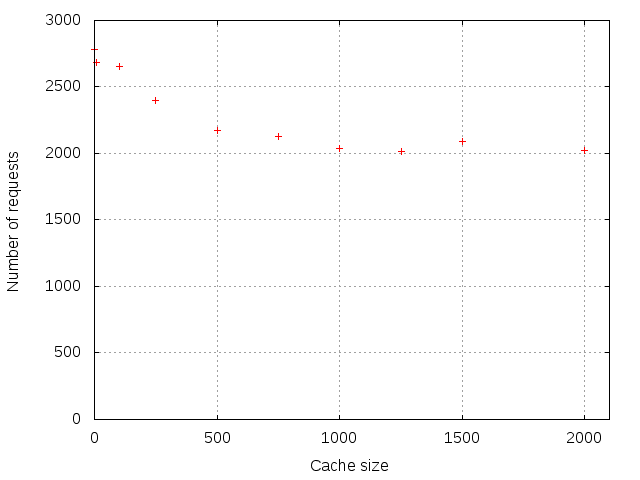
\includegraphics[width=0.9\textwidth]{cache.png}

Please do note, that the number of cache hits in my implementation is not deterministic in nature. This is because all the data points are being calculated concurrently and the order in which the responses arrive from the back end is not deterministic. The trend is quite clear though: increasing cache size will result in fewer requests being sent, which is no surprise. 

\end{document}